\chapter{Prototipazione via Mockup}
I seguenti \textit{Mockup} rappresentano una simulazione grafica delle principali \textbf{interfacce utente} presenti nel sistema.\\
Hanno lo scopo di mostrare in modo chiaro il \textbf{flusso di navigazione} e le \textbf{funzionalità previste} per gli utenti. Le schermate realizzate permettono di visualizzare il \textbf{comportamento del sistema} e l'\textbf{esperienza d'uso} prima di passare all'implementazione effettiva.

\section{Descrizione dettagliata dei Mockup}
\subsection{Schermata di Login}

\begin{figure}[h]
	\centering
	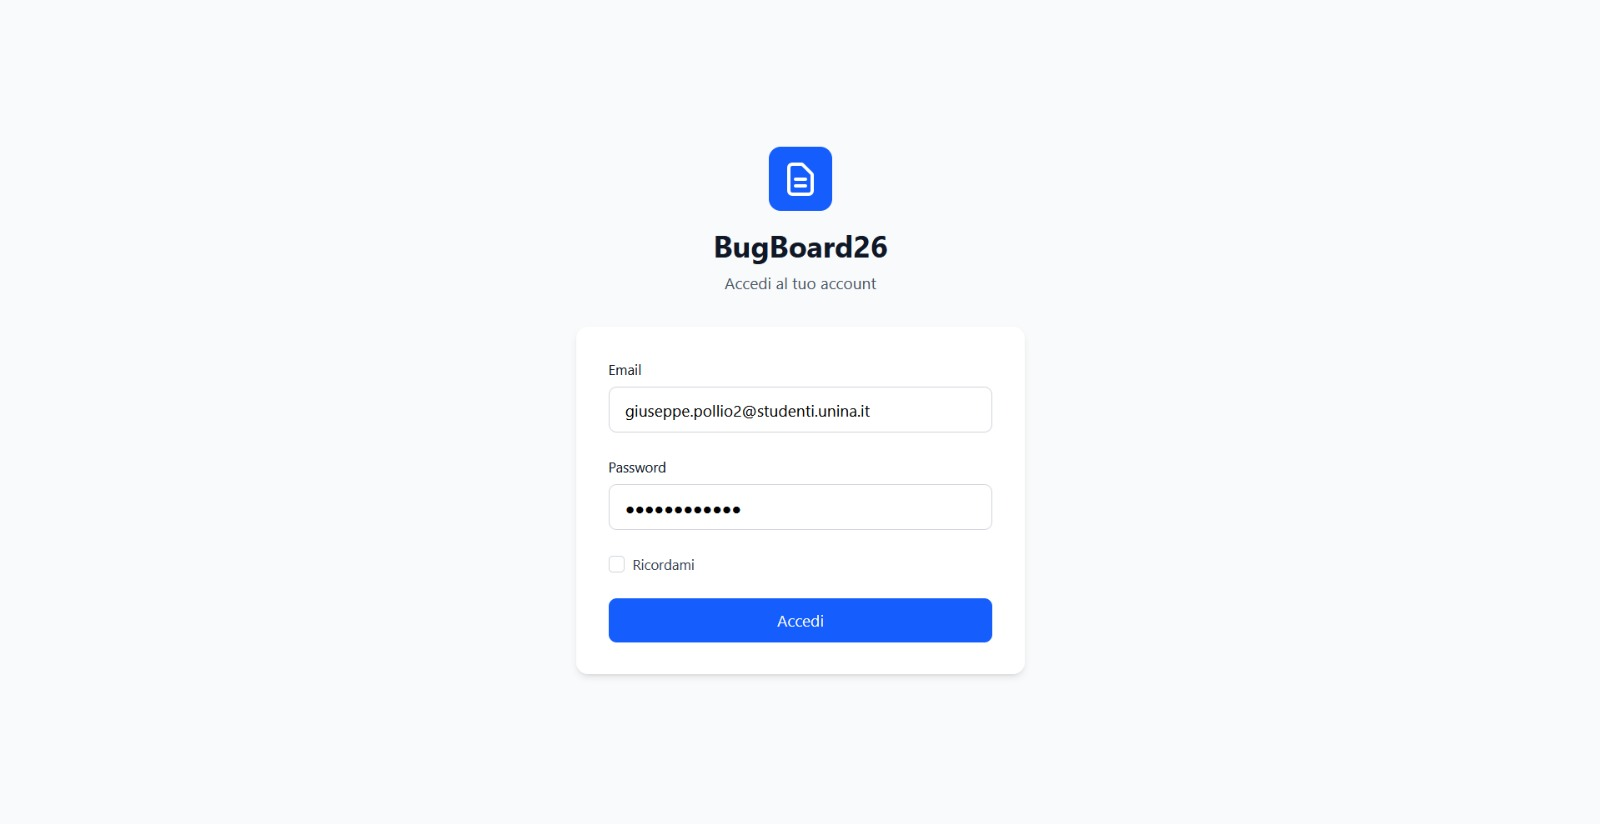
\includegraphics[width=1\linewidth]{./Assets/Chapters/mkp1.jpg}
	\caption{Schermata di login}
\end{figure}

La schermata raffigurata rappresenta la pagina di login al sistema.\\
L'utente da qui inserisce le proprie credenziali per accedere al sistema, scegliendo inoltre se mantenere la sessione attiva tramite la spunta "Ricordami"\\
Una volta autenticato, viene reindirizzato all'\textit{Area progetti}

\subsection{Area progetti}

\begin{figure}
	\centering
	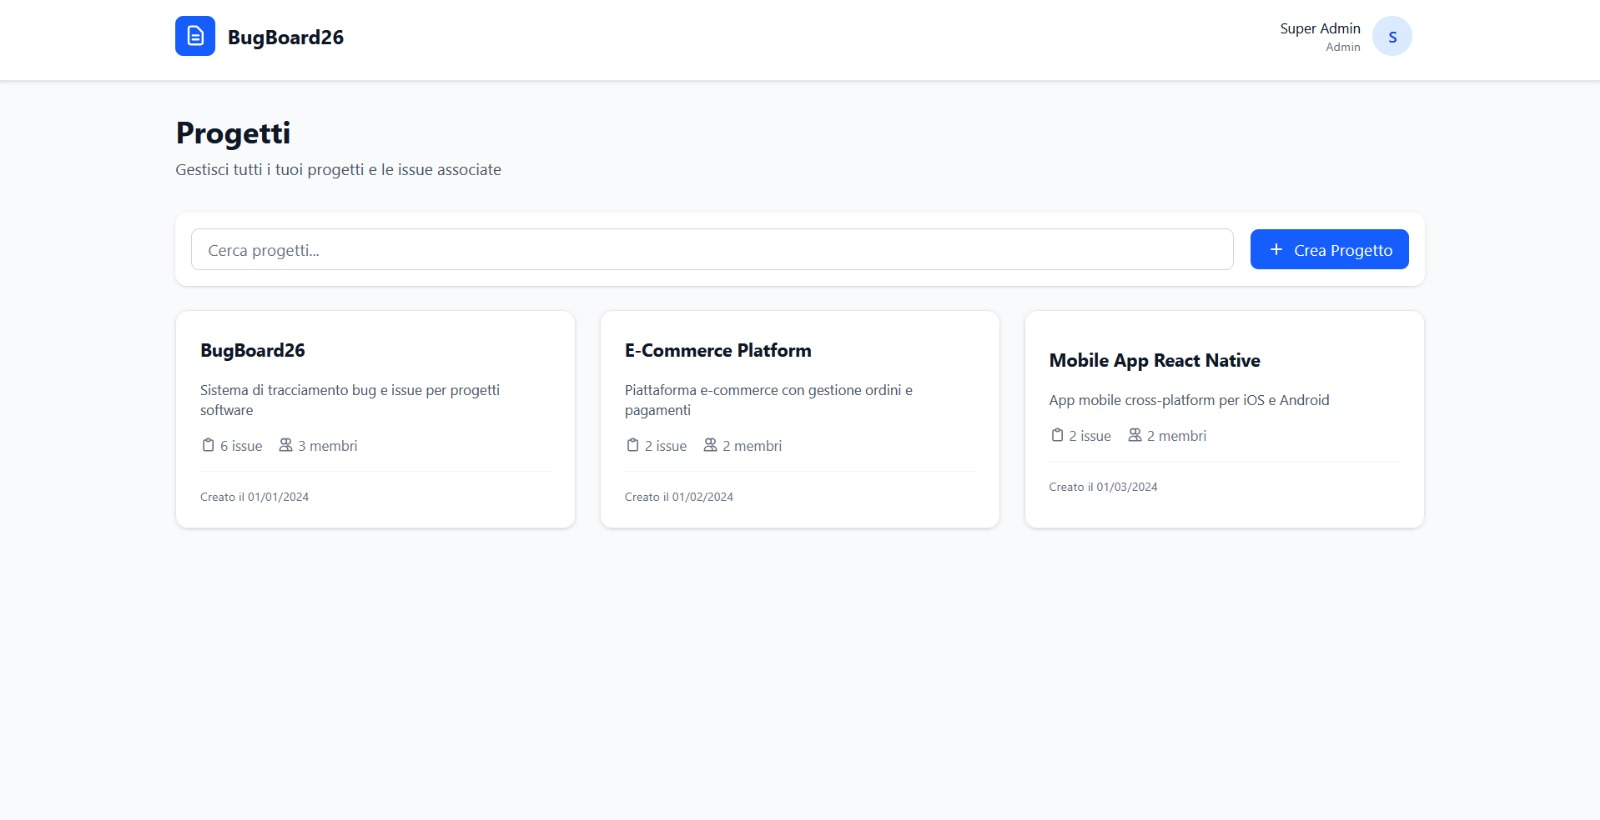
\includegraphics[width=1\linewidth]{./Assets/Chapters/mkp2.jpg}
	\caption{Area progetti}
\end{figure}
Una volta effettuato il login, l'utente accede all'area dei progetti, dove può visualizzare i progetti a cui partecipa.\\
In alto è presente una barra di ricerca per cercare i progetti e un pulsante per crearne di nuovi (visibile solo con account Admin)\\
Ogni progetto è caratterizzato da:
\begin{itemize}
	\item Nome del progetto
	\item Breve descrizione
	\item Numero di \textit{Issue} aperte
	\item Numero di membri del team
	\item Data di creazione
	
\end{itemize}

\subsection{Pagina issues del Progetto}
\begin{figure}
	\centering
	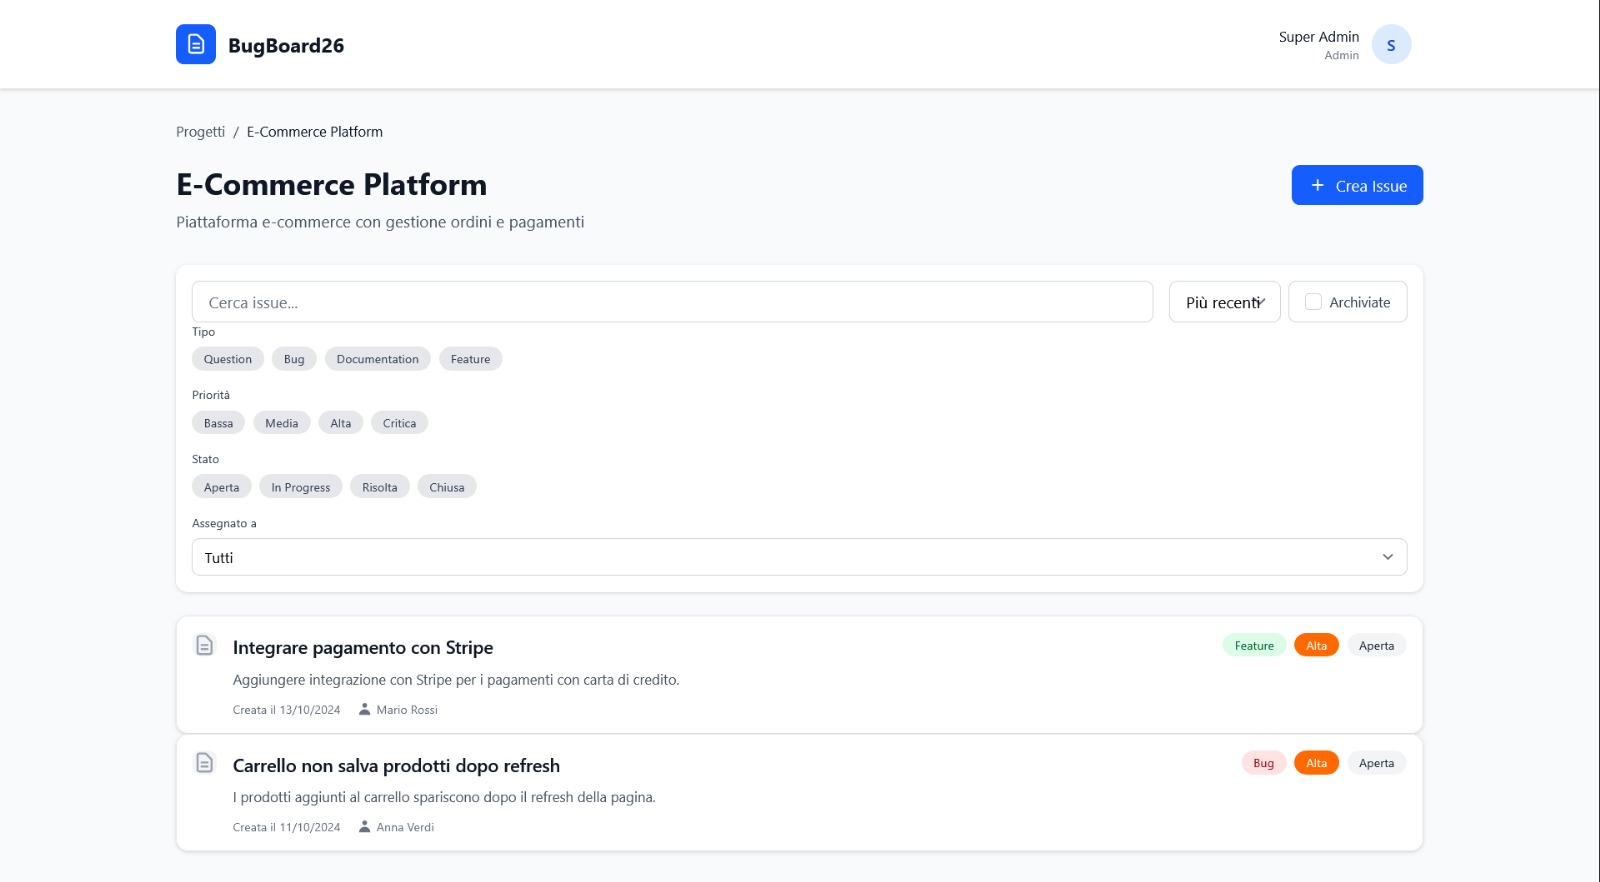
\includegraphics[width=1\linewidth]{./Assets/Chapters/mkp3.jpg}
	\caption{Pagina Issue}s
\end{figure}
Una volta selezionato un progetto, l'utente accede alla pagina delle issues associate.\\
in questa pagina sono visibili tutte le segnalazioni relative al progetto selezionato, con titolo, descrizione, tipo, priorità, stato e autore.\\
Sopra la lista l'utente può filtrare le issues, cercarle nell'apposita barra di ricerca o ordinarle in base alla data di creazione. Inoltre è presente una spunta per visualizzare le issues archiviate.\\
Inoltre è presente il tasto "Crea Issue", che apre il modulo di creazione.


\subsection{Modulo creazione Issue}
\begin{figure}
	\centering
	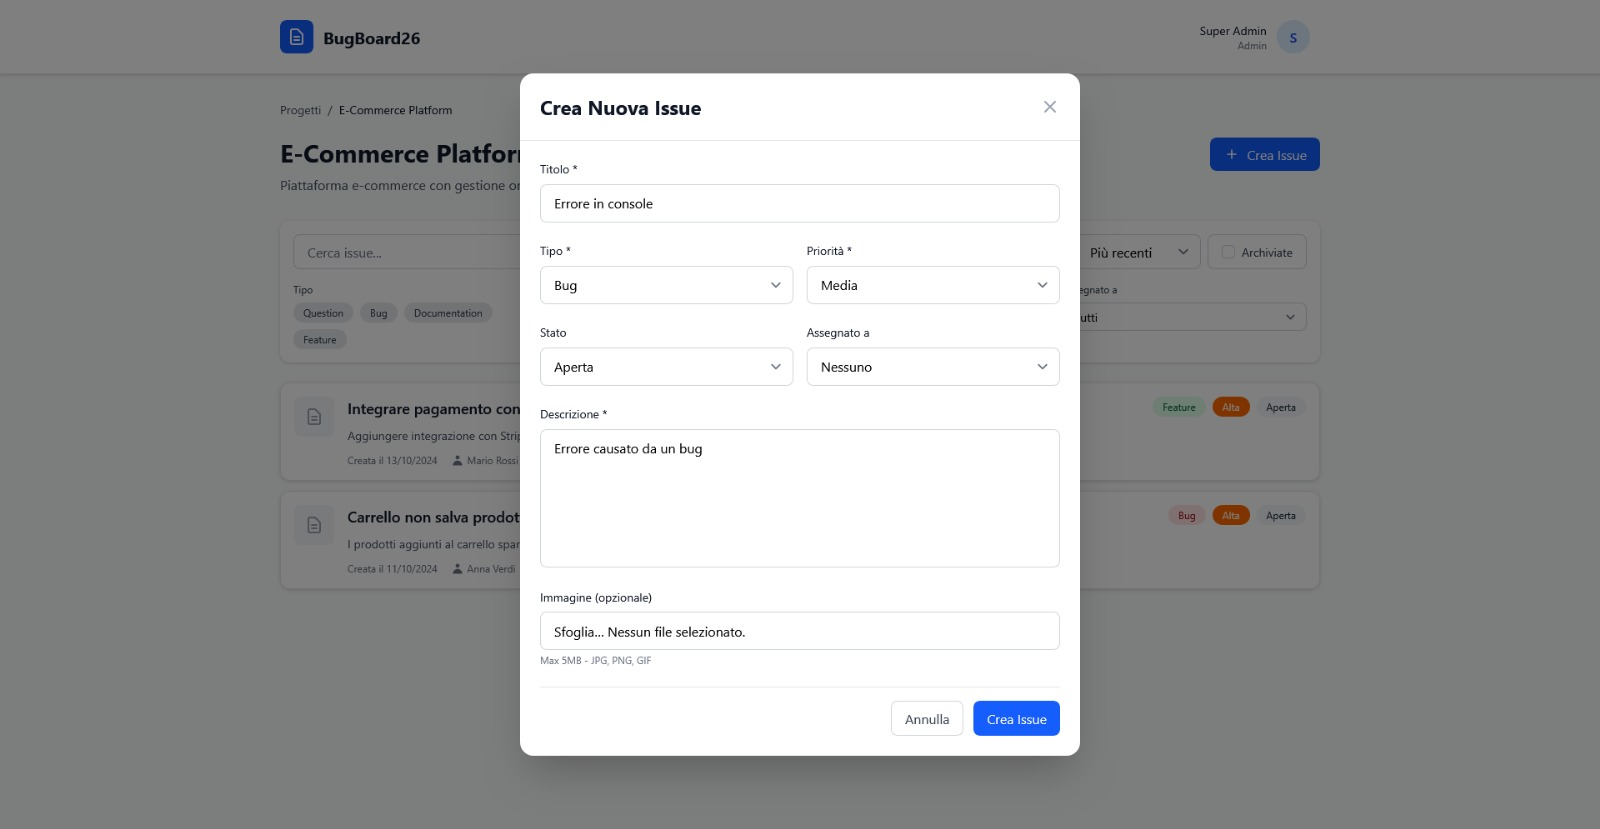
\includegraphics[width=1\linewidth]{./Assets/Chapters/mkp4.jpg}
	\caption{Creazione Issue}
\end{figure}
Il \textit{mockup} sopra mostra il form di inserimento di una nuova \textit{issue}.\\
L'utente deve compilare alcuni campi obbligatori (titolo, tipo, priorità, descrizione), ma può anche aggiungerne di facoltativi (immagine, stato, assegnatario).\\
In fondo al modulo, sono presenti i pulsanti "Annulla" e "Crea Issue", che permettono rispettivamente di chiudere la schermata o di confermare la segnalazione.

\subsection{Aggiornamento lista Issue}
\begin{figure}
	\centering
	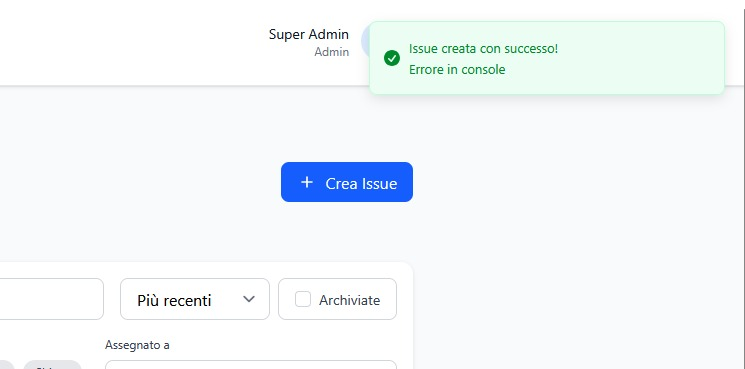
\includegraphics[width=1\linewidth]{./Assets/Chapters/mkp5.jpg}
	\caption{Aggiornamento lista}
\end{figure}
Il \textit{mockup} raffigura la schermata aggiornata dopo la creazione di una nuova \textit{issue}. La lista \textit{issues} viene aggiornata automaticamente con la nuova voce in elenco.\\
Il sistema mostra inoltre una notifica di \textit{feeback} in alto sullo schermo che conferma l'operazione di aggiunta (o segnala un eventuale errore se non è stato possibile aggiungere l'\textit{issue})

\subsection{Errore durante la compilazione del modulo (creazione issue)}
\begin{figure}
	\centering
	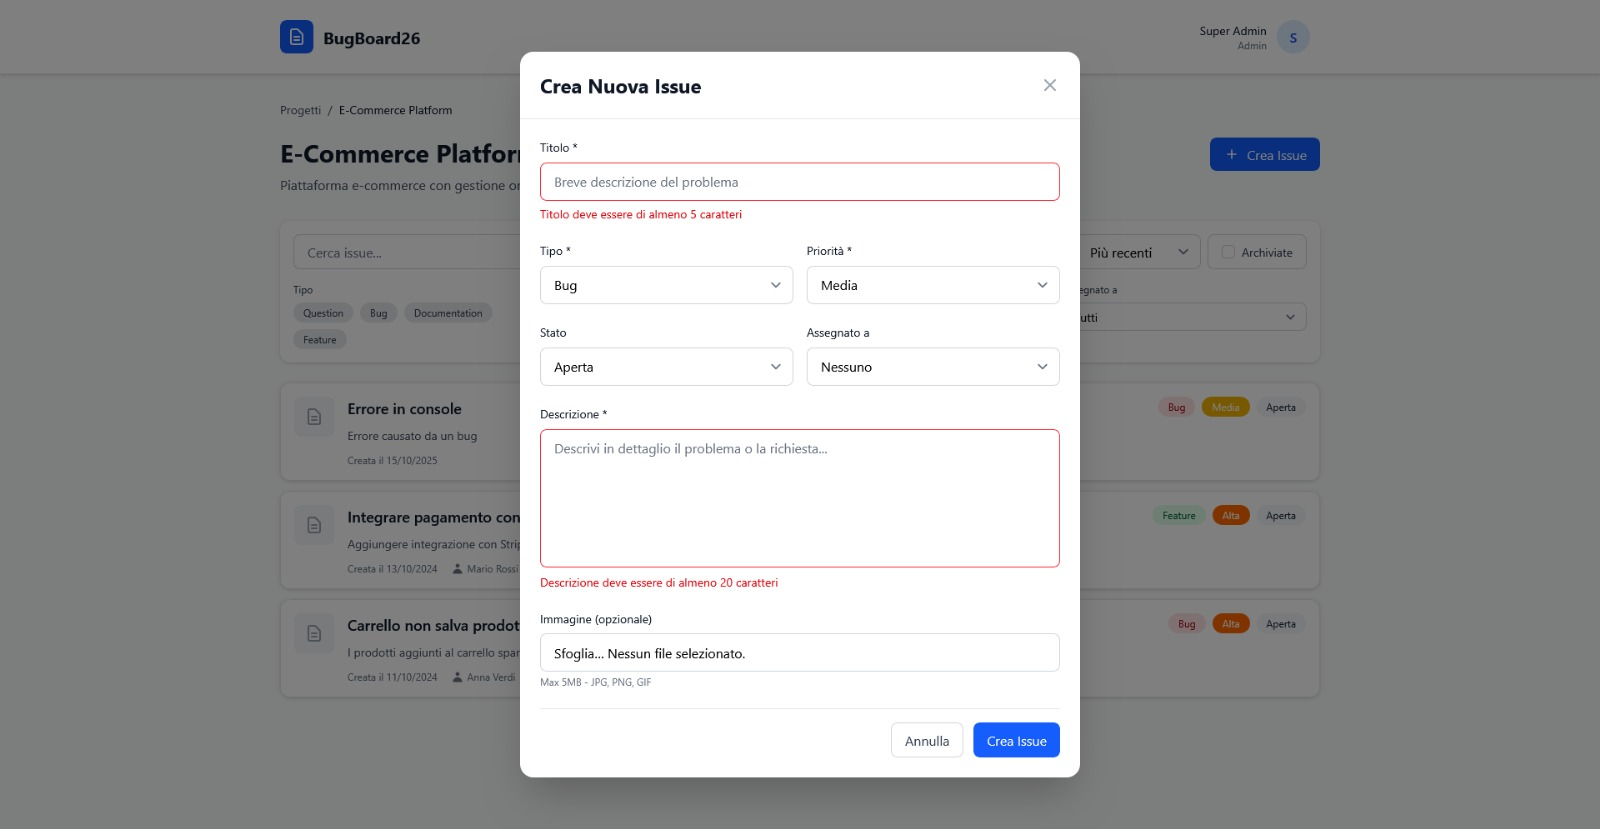
\includegraphics[width=1\linewidth]{./Assets/Chapters/mkp6.jpg}
	\caption{Errore 1}
\end{figure}
Durante la compilazione del modulo, se ci si dimentica di inserire tutti i campi obbligatori, si riscontra il seguente errore. Vengono mostrate i vari messaggi di errore e il sistema aspetta che l'utente corregga l'inserimento dei campi per continuare.

\subsection{Errore interno, per qualche motivo i dati non vengono salvati nel database}
\begin{figure}
	\centering
	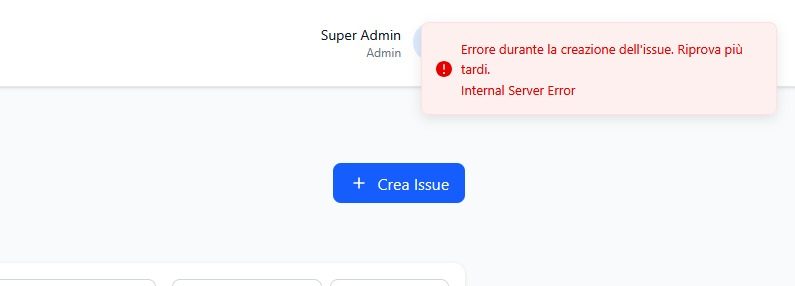
\includegraphics[width=1\linewidth]{./Assets/Chapters/mkp7.jpg}
	\caption{Errore 2}
\end{figure}
Una volta finita la compilazione del modulo, dopo aver premuto il tasto "Crea", se il sistema cade in un qualsiasi errore interno allora viene lanciato il seguente messaggio di errore nella forma di una notifica.
